% TODO :
% ccl



\documentclass[a4paper,11pt]{article}
\usepackage[utf8]{inputenc}
\usepackage{hyperref}
\usepackage{graphicx}
\usepackage[left=2cm,right=2cm,top=2cm,bottom=2cm]{geometry}
\usepackage{fancyhdr}
\usepackage{amsmath,amssymb}


\lhead{\textsc{Introduction to A.I.}}
\rhead{\textsc{Quarto!}}
\cfoot{}
\rfoot{\thepage}
\lfoot{J. Blanchard, A. Deveaux, J. Marnat, C. Schmit}
\renewcommand{\headrulewidth}{.5pt}
\renewcommand{\footrulewidth}{.5pt}
\newcommand{\HRule}{\rule{\linewidth}{0.5pt}}

\newcommand{\tw}[1]{\texttt{#1}}
\newcommand{\mytable}[3]{
	\begin{table}[ht]
		\begin{center}
			\begin{tabular}{#2}
				#3
			\end{tabular}
		\caption{#1}
		\end{center}
	\end{table}
}

\newcommand{\mypic}[3]{
	\begin{picture}[ht]
		\begin{center}
			\includegraphics[#3]{include/#2}
		\caption{#1}
		\end{center}
	\end{picture}
}

\newcommand{\board}[4]{
	\begin{center}
		\begin{tabular}{|c|c|c|c|} \hline
			#1 \\\hline
			#2 \\\hline
			#3 \\\hline
			#4 \\\hline
		\end{tabular}
	\end{center}
}


\begin{document}
	\thispagestyle{empty}
	\vspace{2cm}
	\begin{center}
		\LARGE{\textsc{Université Jean Monnet}}\\[2cm]
		\Large{\textsc{Machine Learning \& Data Mining}} \\[2cm]
		\HRule \\[0.5cm]
		{ \huge \bfseries Introduction to A.I.}\\[0.4cm]
		\textsc{Quarto!}\\
		\HRule \\[1.5cm]
		\normalsize
		\begin{tabular}{r|l}
			Jérémie		& \textsc{Blanchard}\\
			Anthony		& \textsc{Deveaux}\\
			Josselin	& \textsc{Marnat}\\
			Clément		& \textsc{Schmit}	
		\end{tabular}
		\vfill
		
\includegraphics[width=5cm]{include/logoUJM-2016.png}
		\vfill
		2016-2017
	\end{center}
	\newpage

	\renewcommand\contentsname{\begin{center}Table of Contents\end{center}}
	\tableofcontents

	\newpage
	\pagestyle{fancy}

	\section{Introduction}
		We began this project by choosing a game. But it wasn't so easy because we wanted a game that we didn't knew, and a strategical one. After some search: \textsc{Quarto!} came up. A board game with pretty simple rules, and lot of possible strategies. \\
		The first step to test the game was to... have the game! So we have build one in wood, and we started to play lot of time between us, in order to elaborate the strategies we will implement, and become more familiar with the game.

	\section{Presentation of the game}
		\textit{The following description is adapted from the website \href{http://www.ludoteka.com/quarto-en.html}{http://www.ludoteka.com/quarto-en.html}.}

		\paragraph{Origin:} \textsc{Quarto!} is a board game recently invented by Blaise Muller and published by Gigamic

		\paragraph{Description:} This is a game for two players. The board has 16 squares (4x4), and the 16 different pieces that can be constructed combinating the following four characteristics: \tw{colour} (white/black), \tw{size} (long/short), \tw{shape} (round/square), and \tw{hole} (hole/flat).
		
		\paragraph{Objective:} The aim of the game is to complete a line with four pieces that are similar at least about one of the four described characteristics (four big pieces, four little, four red, four blue, four circle, four square, four with hole or four without hole). The line may be vertical, horizontal or diagonal. The winner is the player who places the fourth piece of the line.

		\paragraph{How the game goes on:} Players move alternatively, placing one piece on the board; once inserted, pieces cannot be moved. \\
		One of the more special characteristics of this game is that the choice of the piece to be placed on the board is not made by the same player who places it; it is the opponent who, after doing his move, decides which will be the next piece to place. \\
		So, each turn consists of two actions: 1. Place on the board the piece given by the opponent. 2. Give to the opponent the piece to be placed in the next move. \\
		In the first turn of the game, the player who starts has only to choose one piece for the opponent.

		\paragraph{Final:} The game finishes in a draw when nobody reaches the objective after placing the 16 pieces.

	\section{How to run the program and play}
		\begin{enumerate}
			\item First, open a terminal and change your current working directory to the one who contains the files \tw{main.pl}, \tw{quarto.pl}, \textit{etc.};
			\item Then, run your \textsc{Prolog} machine, and consult the main file by typping `\tw{[main].}'
			\item Finally, you can run the game by calling the predicate `\tw{play(Interface,Heuristics1,Heuristics2)'}. (type `\tw{how\_to\_play.}' for further informations).
			\item If one of your heuristics are \tw{human}, it'll be asked to you to input a \tw{PieceID}, and later a position \tw{[Row,Col]}, until the game ends.
		\end{enumerate}


	\section{The game-play algorithm}
		If you look at the file named \tw{quarto.pl}, you'll see the following predicate:\\
			\tw{play(Interface,Heuristics1,Heuristics2)},\\
		who are running the game. \\
		But the actual predicate who does the job is \tw{round(Interface,...)}, and here is how it works:
		\begin{enumerate}
			\item first, we check if somebody wins $\rightarrow$ \textsc{Game Over}
			\item then, we check if the board is full $\rightarrow$ \textsc{Game Over}
			\item if none of this first predicates come \tw{true}, we launch a round, splitted in two parts:
			\begin{enumerate}
				\item first part: the player need to choose a piece:
				\begin{itemize}
					\item we display the board, the player, the pieces \textit{etc.} ;
					\item we ask a piece to the player (human or computer) ;
				\end{itemize}
				\item we swap the players to do the second part of the round:
				\begin{itemize}
					\item we display the piece to play;
					\item we read the position where the player want to put the given piece;
					\item then, we put the piece on the board (by getting a \tw{NewBoard});
					\item finally, we run a new round with the baord obtained (return to 1.).
				\end{itemize}
			\end{enumerate}
		\end{enumerate}

	\section{Heuristics}
		\paragraph{Random (\tw{random.pl}):} this heuristics is the `stupid' one. \\
		It selects a piece randomly among the available ones, and do the same thing for the position. This heuristics was created at the very beggining of the project, just to test the game-play, and to have a base to create the other ones.
		
		\textit{The following descriptions of the heuristics have been written by each team member.}
		
		\paragraph{Anthony (\tw{anthony.pl}):} The AI prepare the Board for the first 5 turn, minimizing the number of alignment between each pieces in the board, and by giving pieces sharing the fewer attributes with the piece the AI receive. \\
		Why the five first turn are preparing the board? Because when you mimizing the number of alignement the fifth turn can share attributes between 2 and more lines. Thanks to all pieces giving because you giving all pieces that sharing fewer attributes as possible and the opponement have to pose them choosing by align with other pieces and not. In wich case it can helps us to do more alignement. \\
		For next turns, the AI became more agressive by giving non loosing pieces and maximizing the number of attributes share with the last piece receive by the AI. And choosing position where we can maximizing the number of share aligments with the maximum of share. If the Board is too bad the AI (loosing next turn), then the AI play in a position that can free some pieces to give and possibly can switch the Board into good board (winning next turn).

		\paragraph{Josselin (\tw{josselin.pl}):} The idea of this AI is of course to get the piece and position to play each round. I's a simplified version of minimax: we don't build and search any tree, we just try to get a winning piece/position. \\
		First, we're searching for the piece which is associated with the biggest value (or score). The values are distributed from the highest to the lowest according this rules: we are shure to win; we coul'd win the next round; the other player can't win next round; random selection. And it's the same kind of association for the positions. \\
		The idea is that to check if we are shure to win with a piece, we check that, for all positions selected by the adversary, whatever the piece he gives us after putting his on the board, we can win with it.

		\paragraph{Clément (\tw{clement.pl}):} A main predicate is used in this heuristic. This is the ListWin predicate it goes through all the board and look for winning pieces. These winning positions are put in a list (coordinates with winning caracteristics). \\
		When you need to place the piece that was given to you, the read position predicate look for a position where the piece can win if placed there. \\
		On the other way when you need to choose a piece for your opponnent you use again the ListWin but this time the piece you give must not have a common caracteristics with one of the winnings piece in the ListWin so that your opponent can't win with this piece on his turn. \\
		Example :
		\board{1 & 0 & 0 & 10}{0 & 2 & 11 & 0}{0 & 0 & 3 & 0}{12 & 0 & 0 & 0}
		With this board the winlist is:\\
		\tw{[[white, 4, 4], [short, 4, 4], [black, 3, 2], [short, 3, 2]]} \\
		You can win by either placing a white piece in 4,4 or a short one in 4,4 \textit{etc.}\\
		In this board we cannot find a piece to win we have to loose considering there is a winnable position with a black piece and a white piece. Considering a piece is either white or black there is no solution. \\
		In this case we call a random piece because the previous predicate will fail. \\
		Exemple: \board{1 & 0 & 0 & 10}{0 & 2 & 11 & 0}{0 & 0 & 0 & 0}{12 & 0 & 0 & 0}
		With this board the winlist is \tw{[[black, 3, 2], [short, 3, 2]]} \\
		So after placing the piece we would choose one that doesn't allow our opponnent to win. \\
		In this case we need a piece that isn't black or that isn't short.
		
		\paragraph{Jérémie (\tw{jeremie.pl}):} To make this IA, I decided to create a Min Max algorithm which takes the best position option for the given piece, and gives the enemy a piece that will make him less likely to win. In order to do that I had to calculate the weight of every playable board to know which one I had to choose. To calculate the weight I simply took the board of which I wanted to know the weight, and added up all the characteristics of all the pieces on the board one by one. Then I had to compare them with each other to take the minimal one. Once I had done that for one board, I had to do it for all the other boards that are linked to the original board, and put the minimal value of each one into a list, and finally I took the minimal value of this list. Then I picked the board that had this minimal value. \\
		To know which piece I have to give my opponent, I used the same system as before, but this time I took the board with the highest weight.

	
	\section{User Interfaces}
		\subsection{Inline mode}
			The first interface, and still the efficient one, is the 'inline-mode' interface. Each round, we print in the terminal the board with the pieces described as binary values (0 or 1 for each attribute), display the available pieces, ask for a piece, and a position to the adversary. 

		\subsection{GUI: an XPCE (mis)adventure...}
			Since \textsc{Prolog} is a pretty ``outside the box'' language, there isn't a lot of libraries who allows it to make a proper GUI with interactions. \\
			I decided to use the only library who worked for me: \textsc{XPCE}, and after \textbf{a lot of time}, I was able to display the window with the board and the pieces, and trigger predicated by clicking on the cells or the pieces. But get the triggers into the execution of the rounds was just impossible. We can't say to \textsc{Prolog}: ``wait for somebody to click in the window and continue the round''. So at the end, I wasn't able to do that after all this time to try. \\
			The fact is that we can actually output the number of the piece clicked into the terminal, and a line return to emulate a physical user, but \textsc{Prolog} do not recognize it as an actual input, while waiting for an \tw{read()}. \\
			Though, I wouldn't consider it as a failure, because maybe there is a way to make it work, but it still not a full graphical interface. \\
			If you want to try the UI on your computer, you need to run it either on Linux, or on Mac (having \textsc{XQuartz} installed before). And you must type `\tw{free.}' in before quitting prolog to dismiss the window.
	
	\section{Tests, efficiency and challenges}	
		\subsection{Statistics foreach heuristics}
			The predicate \tw{time(.)} displays some informations about the execution of a predicate. \\
			We use it in \tw{stats(Heuristics1,Heuristics2,NumTime)} to run the game between this two heuristics, a \tw{NumTime} number of time, and then it will display who won how many time (with \tw{test\_play(...)}), and the number	of inferences, the CPU usage and the time of the execution. With this predicate, we were able to ran 100 times the game with each pair of heuristics we've made (exept for \tw{human}). Then, we've put the data in the three following tables for comparison.

			\mytable{Number of wins for 100 iterations}{|l||r|r|r|r|r|}{
				\hline
				\#Wins		& random	& anthony	& josselin	& clement	& jeremie	\\\hline\hline
				random		& 50		& 2			& 1			& 32		& 44		\\\hline
				anthony		& 100		& 29		& 68		& 100		& 99		\\\hline
				josselin	& 100		& 4			& 100		& 99		& 76		\\\hline
				clement		& 58		& 29		& 25		& 55		& 53		\\\hline
				jeremie		& 47		& 0			& 0			& 41		& 62		\\\hline
			}

			\mytable{Execution time for 100 iterations}{|l||r|r|r|r|r|}{
				\hline
				Time		& random	& anthony	& josselin		& clement	& jeremie	\\\hline\hline
				random		& .4 s		& 4 s		& 33 s			& 0.8 s		& 102 s		\\\hline
				anthony		& 4 s		& 43 s		& 49 s			& 4 s		& 81 s		\\\hline
				josselin	& 39 s		& 48 s		& 89 s			& 39 s		& 147 s		\\\hline
				clement		& .7 s		& 4 s		& 34 s			& 1 s		& 117 s		\\\hline
				jeremie		& 87 s		& 75 s		& 109 s			& 77 s		& 116 s		\\\hline
			}

			\mytable{Number of inferences for 100 iterations (M = $10^6$)}{|l||r|r|r|r|r|}{
				\hline
				Inferences		& random	& anthony	& josselin	& clement	& jeremie	\\\hline\hline
				random			& 2 M		& 36 M		& 304 M		& 5 M		& 185 M		\\\hline
				anthony			& 34 M		& 398 M		& 445 M		& 39 M		& 206 M		\\\hline
				josselin		& 341 M		& 430 M		& 827 M		& 342 M		& 530 M		\\\hline
				clement			& 5 M		& 38 M		& 315 M		& 8 M		& 188 M		\\\hline
				jeremie			& 149 M		& 171 M		& 419 M		& 149 M		& 271 M		\\\hline
			}

			And we don't have to say much about it, the data speaks by itself... \\
			Maybe we could just say that even if there are very big numbers in this tables, espacially in time, it's important to remark that it is for a hundred of fully-executed games. So in fact, the time response of the AI when playing a normal game (against an human) is most of the time not even noticeable.
		
		\subsection{Challenges and difficulties}
			\paragraph{Jérémie: } During this project I encountered a lot of issues, but most of them were issues cause by the difference between \textsc{Prolog}, and other languages that I was used to use during my bachelor. So it was hard to me to visualize how a list can behave, where I have to add bracket or where I have to remove them. Managing the lists was the most difficult things, with writing every function in a recursive way.

			\paragraph{Josselin:} At the beggining, my heuristics was supposed to be based on a minimax algorithm. I implemented it a few times in other languages and it doesn't seemed to complicated. But the way our \textsc{Quarto!} is implemented made this more difficult than explected, so I rethought all my code and simplified it a lot. \\
			Build the evaluation and scoring predicates recursively was really hard and I decided to make it simpler just by checking on a few rounds by hand. \\
			The other main difficuly I faced of is the GUI. I really passed a huge amount of time to test a lot of different things to try to make it work, but unsuccessfully

			\paragraph{Clément:} During the creation of this heuristic I get to meet some difficulties on the \tw{winlist} creation and stop point. Especially in the case where there is no solution for the predicate. You have to choose for a random position if not the predicate returns \tw{false}. Example if there is no winning position, \tw{WinList} is then empty so the predicate have to choose a random solution

			\paragraph{Anthony:} The biggest problem was to elaborate this strategy, because I have to do a lot a test by playing (against real players). And the problem that take me most of my time was to find a way of coding my strategy. So again lot of test and try to correct all errors I have made and after, optimizing the code and try to have better score. And the last was to found an optimization of sharing attributes with a piece.
	
	\section{Conclusion}
		This project was interesting from many point of views. First, we had to immerge us totally in the ``\textsc{Prolog} world'', because it's like any other languages we know. Writing algorithms only by saying things that are true is a very unusual way to think a program. Some of us didn't knew this language before and in this way it was a real challenge. \\
		Moreover, having four different heuristics was at the same time a bit complicated (we needed to be very creative), but interesting as well because each of us had a very different view on how to implement a powerful AI against the adversary. \\
		Finally, we ended up with pretty nice heuristics who will for sure beat a ordinary human a lot of times (especially since humans do mistakes!).

		\vfill
		\begin{flushright}
			\footnotesize{Written in \LaTeX\ by J. \textsc{Marnat} $\blacksquare$}
		\end{flushright}

	\newpage
	\section{Appendices}
		\mytable{Approximate time for coding each files}{|l||l|r|}{\hline
			\tw{quarto.pl}				& Josselin		& 10-12 h	\\\hline
			\tw{inline\_interface.pl}	& Josselin		& 3-4 h		\\\hline
			\tw{gui.pl}					& Josselin		& 5-7 h		\\\hline
			\tw{random.pl}				& Josselin		& 5 m		\\\hline
			\tw{human.pl}				& Josselin		& 15 m		\\\hline
			\tw{anthony.pl}				& Anthony		& 25-30 h	\\\hline
			\tw{clement.pl}				& Clément		& 12-15 h	\\\hline
			\tw{jeremie.pl}				& Jérémie		& 30-35 h	\\\hline
			\tw{josselin.pl}			& Josselin		& 8-10 h	\\\hline
		}

		\begin{figure}[ht]
			\begin{center}
				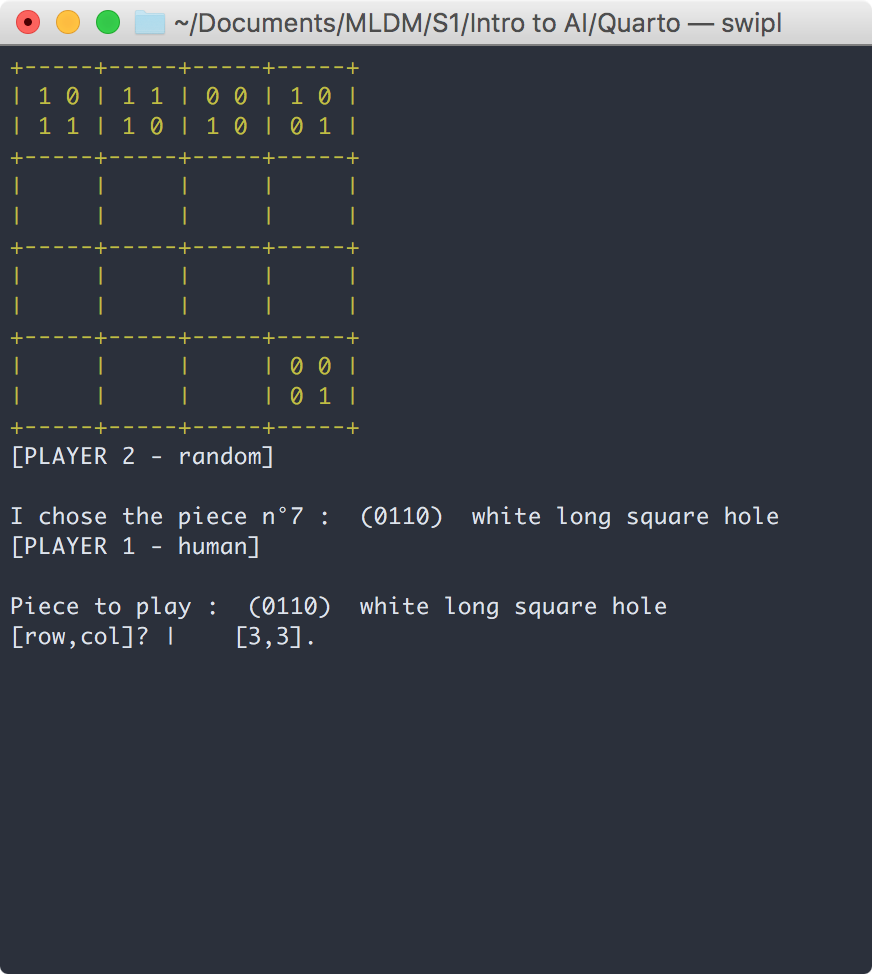
\includegraphics[width=5cm]{include/inline1.png}
				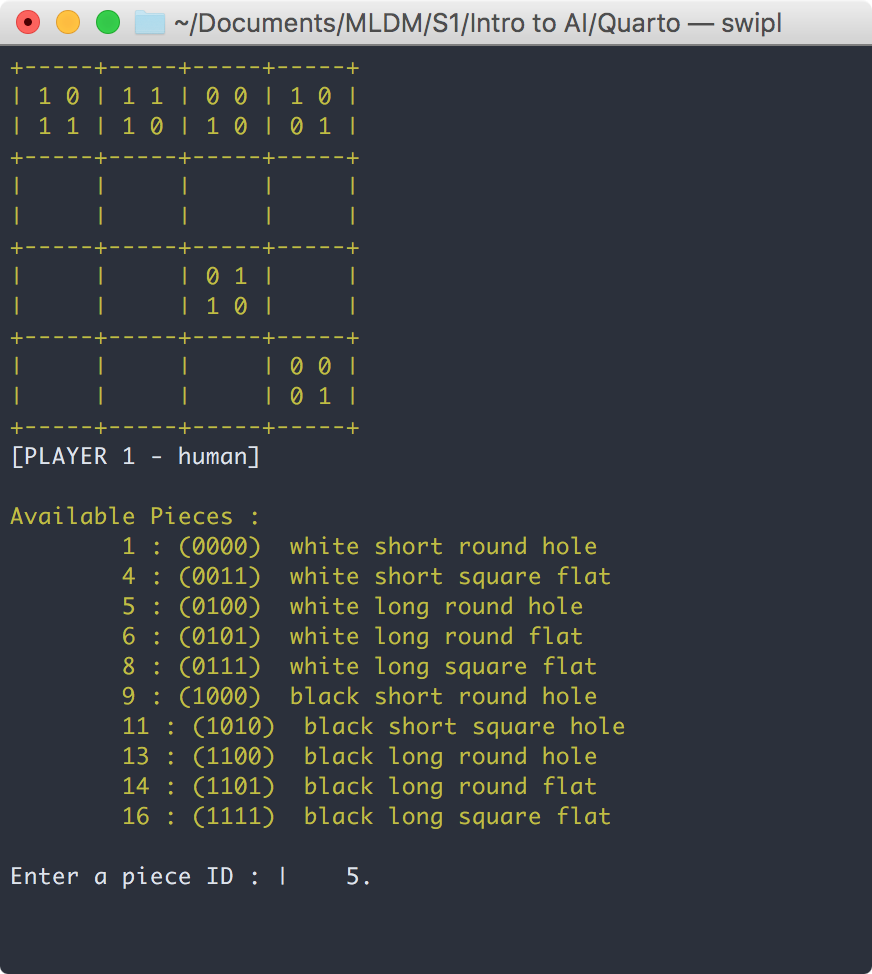
\includegraphics[width=5cm]{include/inline2.png}
				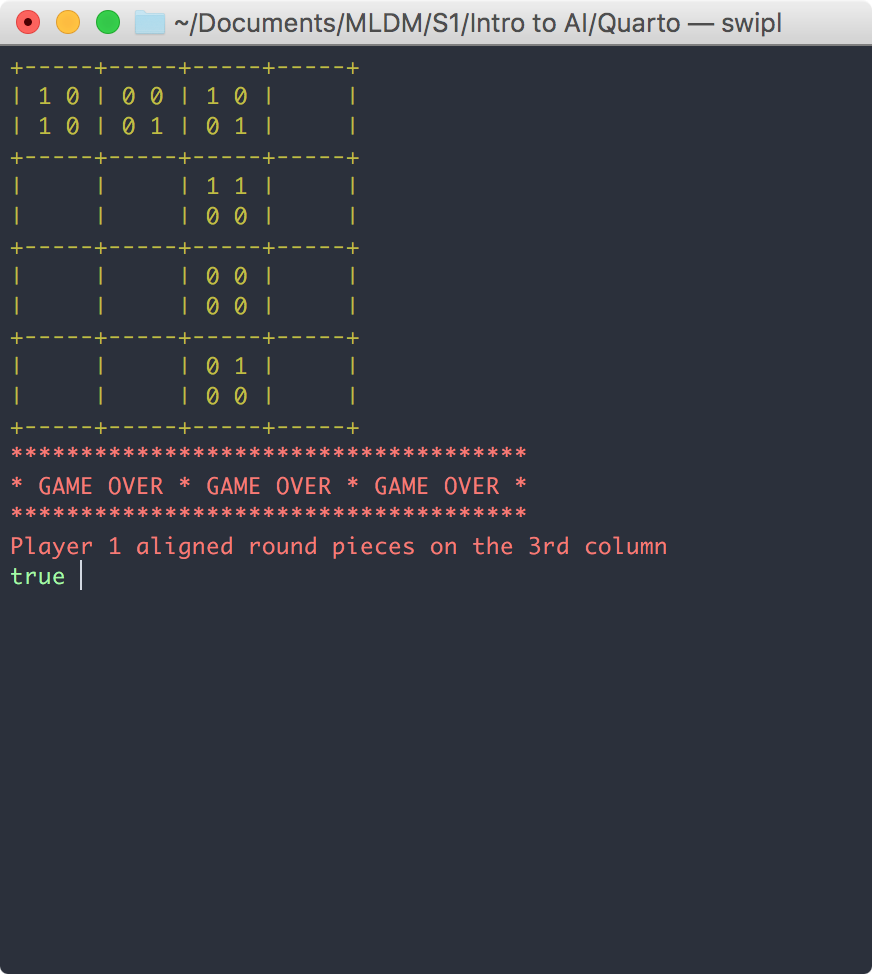
\includegraphics[width=5cm]{include/inline3.png}
			\caption{The inline interface}
			\end{center}
		\end{figure}

		\begin{figure}[ht]
			\begin{center}
				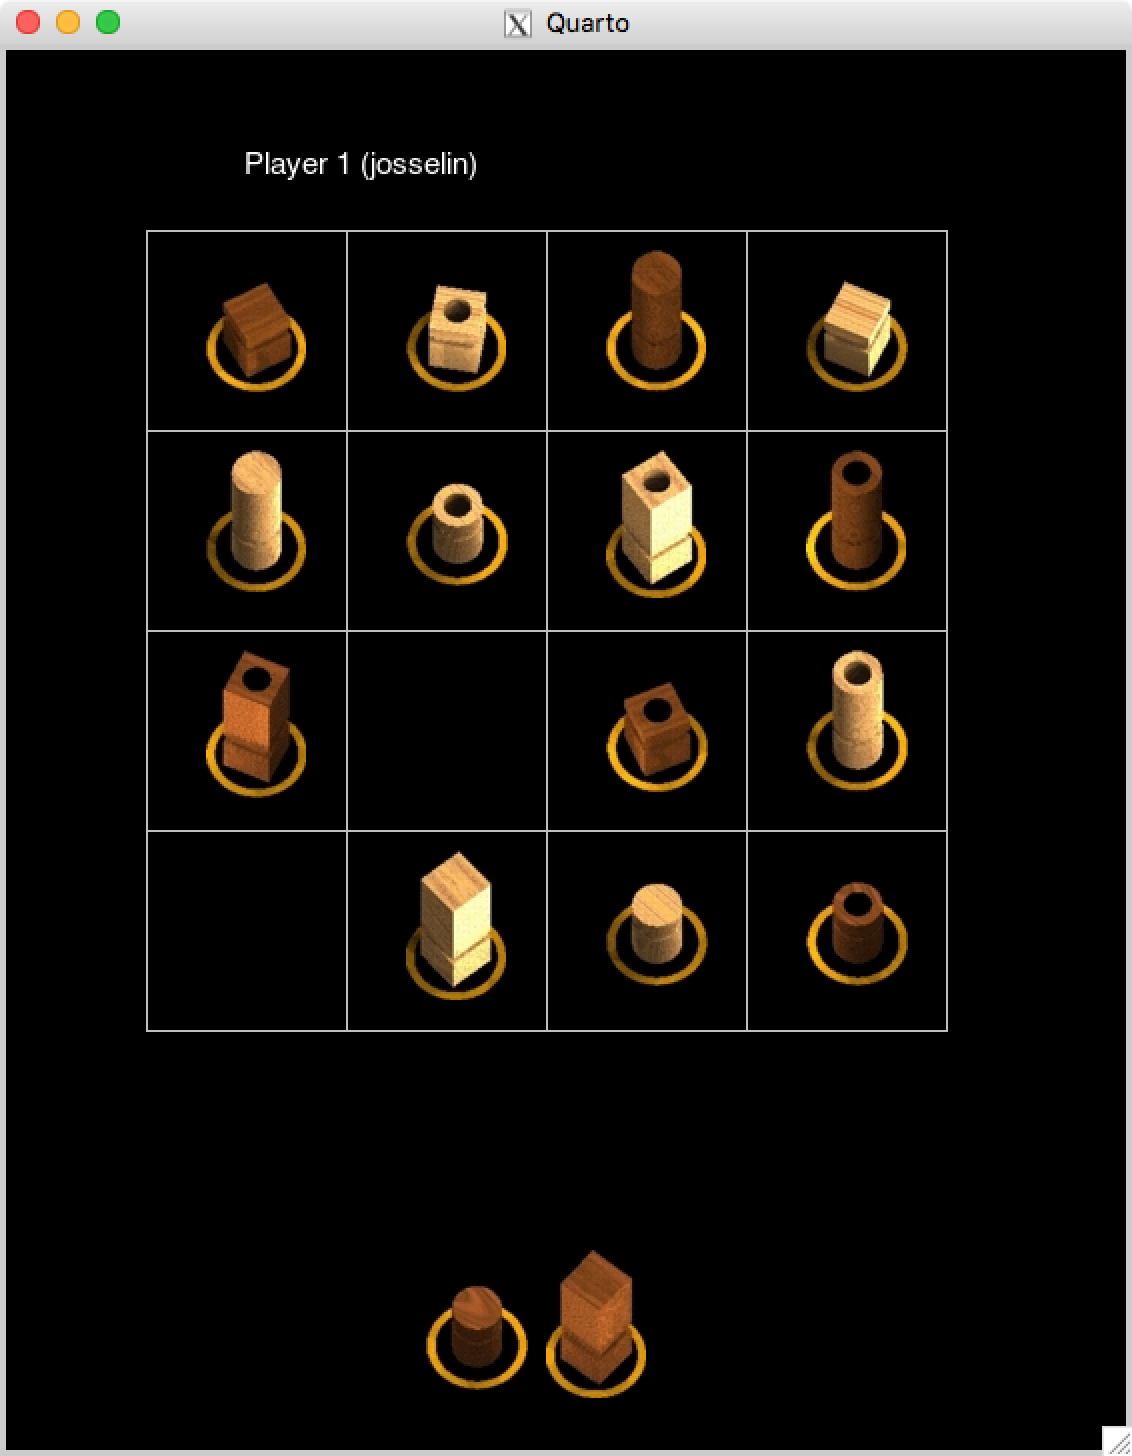
\includegraphics[width=9cm]{include/gui1.png}
				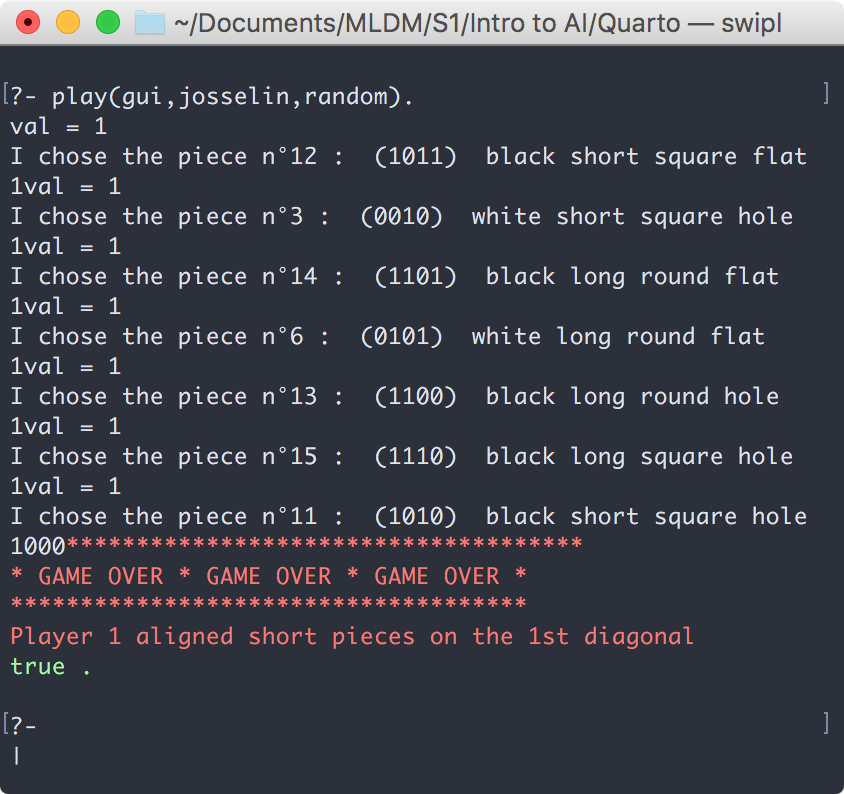
\includegraphics[width=6cm]{include/gui2.png}
			\caption{The GUI along the terminal}
			\end{center}
		\end{figure}

		\begin{figure}[ht]
			\begin{center}
				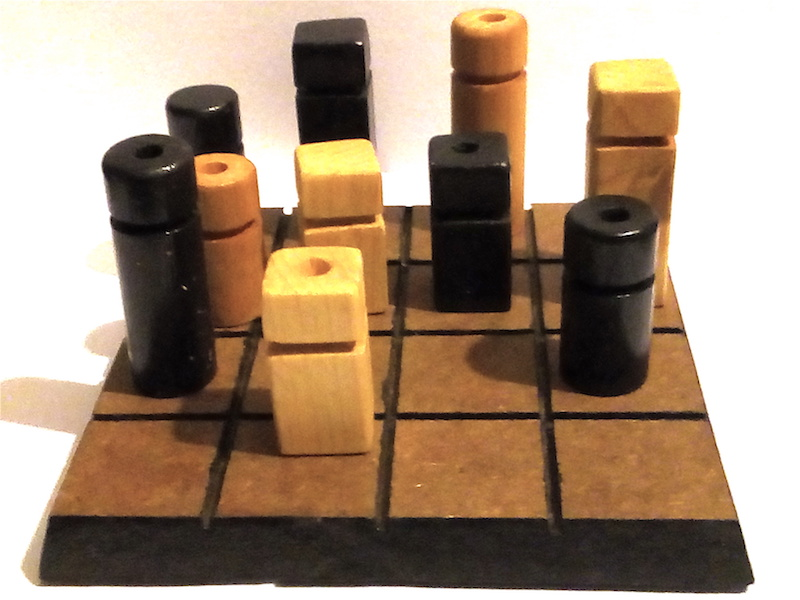
\includegraphics[width=\linewidth]{include/homemade-quarto.jpg}
			\end{center}
			\caption{My homemade wooden \textsc{Quarto!}}
		\end{figure}


\end{document}
